%%%%%%%%%%%%%%%%%%%%%%%%%%%%%%%%%%%%%%%%%
% Memo
% LaTeX Template
% Version 1.0 (30/12/13)
%
% This template has been downloaded from:
% http://www.LaTeXTemplates.com
%
% Original author:
% Rob Oakes (http://www.oak-tree.us) with modifications by:
% Vel (vel@latextemplates.com)
%
% License:
% CC BY-NC-SA 3.0 (http://creativecommons.org/licenses/by-nc-sa/3.0/)
%
%%%%%%%%%%%%%%%%%%%%%%%%%%%%%%%%%%%%%%%%%

\documentclass[letterpaper,11pt]{texMemo} % Set the paper size (letterpaper, a4paper, etc) and font size (10pt, 11pt or 12pt)

\usepackage{parskip} % Adds spacing between paragraphs
\usepackage[colorlinks]{hyperref}
\usepackage{graphicx}
\usepackage{float}
\usepackage{hyperref}
\usepackage{listings}
\hypersetup{citecolor=DeepPink4}
\hypersetup{linkcolor=red}
\hypersetup{urlcolor=blue}
\usepackage{cleveref}
\setlength{\parindent}{15pt} % Indent paragraphs

%----------------------------------------------------------------------------------------
%	MEMO INFORMATION
%----------------------------------------------------------------------------------------

\memoto{Dr.Randy Hoover} % Recipient(s)

\memofrom{Benjamin LeBrun, Benjamin Garcia} % Sender(s)

\memosubject{Lab Assignment 5: Timers and Motor Control} % Memo subject

\memodate{\today} % Date, set to \today for automatically printing todays date

% \logo{\includegraphics[width=0.1\textwidth]{logo.png}} % Institution logo at the top right of the memo, comment out this line for no logo

%----------------------------------------------------------------------------------------

\begin{document}

\maketitle % Print the memo header information

%----------------------------------------------------------------------------------------
%	MEMO CONTENT
%----------------------------------------------------------------------------------------

\section*{Introduction}
For this lab, we utilized the full car kit of our Elegoo robot package to 
explore using power width modulation (PWM) to send a controlled motor signal to an H-bridge chip
and drive a set of DC motors with two separate channels. This required the
use of writing to the Atmega328p's internal timers to prevent overloading or locking
the CPU with delay signals or other inefficient methods.

\section*{Equipment}
While the lab used the entire robot kit assembled together, the primary devices
we used were:

\begin{itemize}
    \item Acrylic vehicle body with screws, assembled
    \item Elegoo Uno (chip: Atmega328p)
    \item 4 DC motors with wheels, screws 
    \item L298 H bridge module dual channel
    \item 2 ICR18650 batteries with battery box
    \item Ribbon cables
    \item Host laptop with AVR-gcc 8-bit toolchain
    \item USB 2.0 A to B cable
\end{itemize}

\subsection*{Configuration}
Our robot vehicle was assembled according to Elegoo's instructions which can be found
on Elegoo's website at \url{https://www.elegoo.com/download/}. For this lab, we are
using the V3.0 version of the robot kit.

The components in the kit have a clearly marked port on the Arduino shield included in 
the package. This makes it easier to identify and connect together ports using the also 
included ribbon cables with some degree of cable management. One of the early pitfalls is
that the H bridge connector is a six pin ribbon cable, which to the uncareful eye looks like 
the five pin cable connector between the shield board and the line following IR sensors.

Besides the ribbon cable for our ports, we also have a DC cable to power the H bridge driver. 
This is because the DC motors have massively larger power requirements (up to a maximum of 2 amps) 
than our Arduino (40 milliamps maximum, both at 5 volts). Therefore, the external batteries are 
required to power the DC motors via the H bridge separate from the Arduino. Wheels were also attached 
and secured with standard phillips head screws.

\begin{figure}[!ht]
\begin{center}
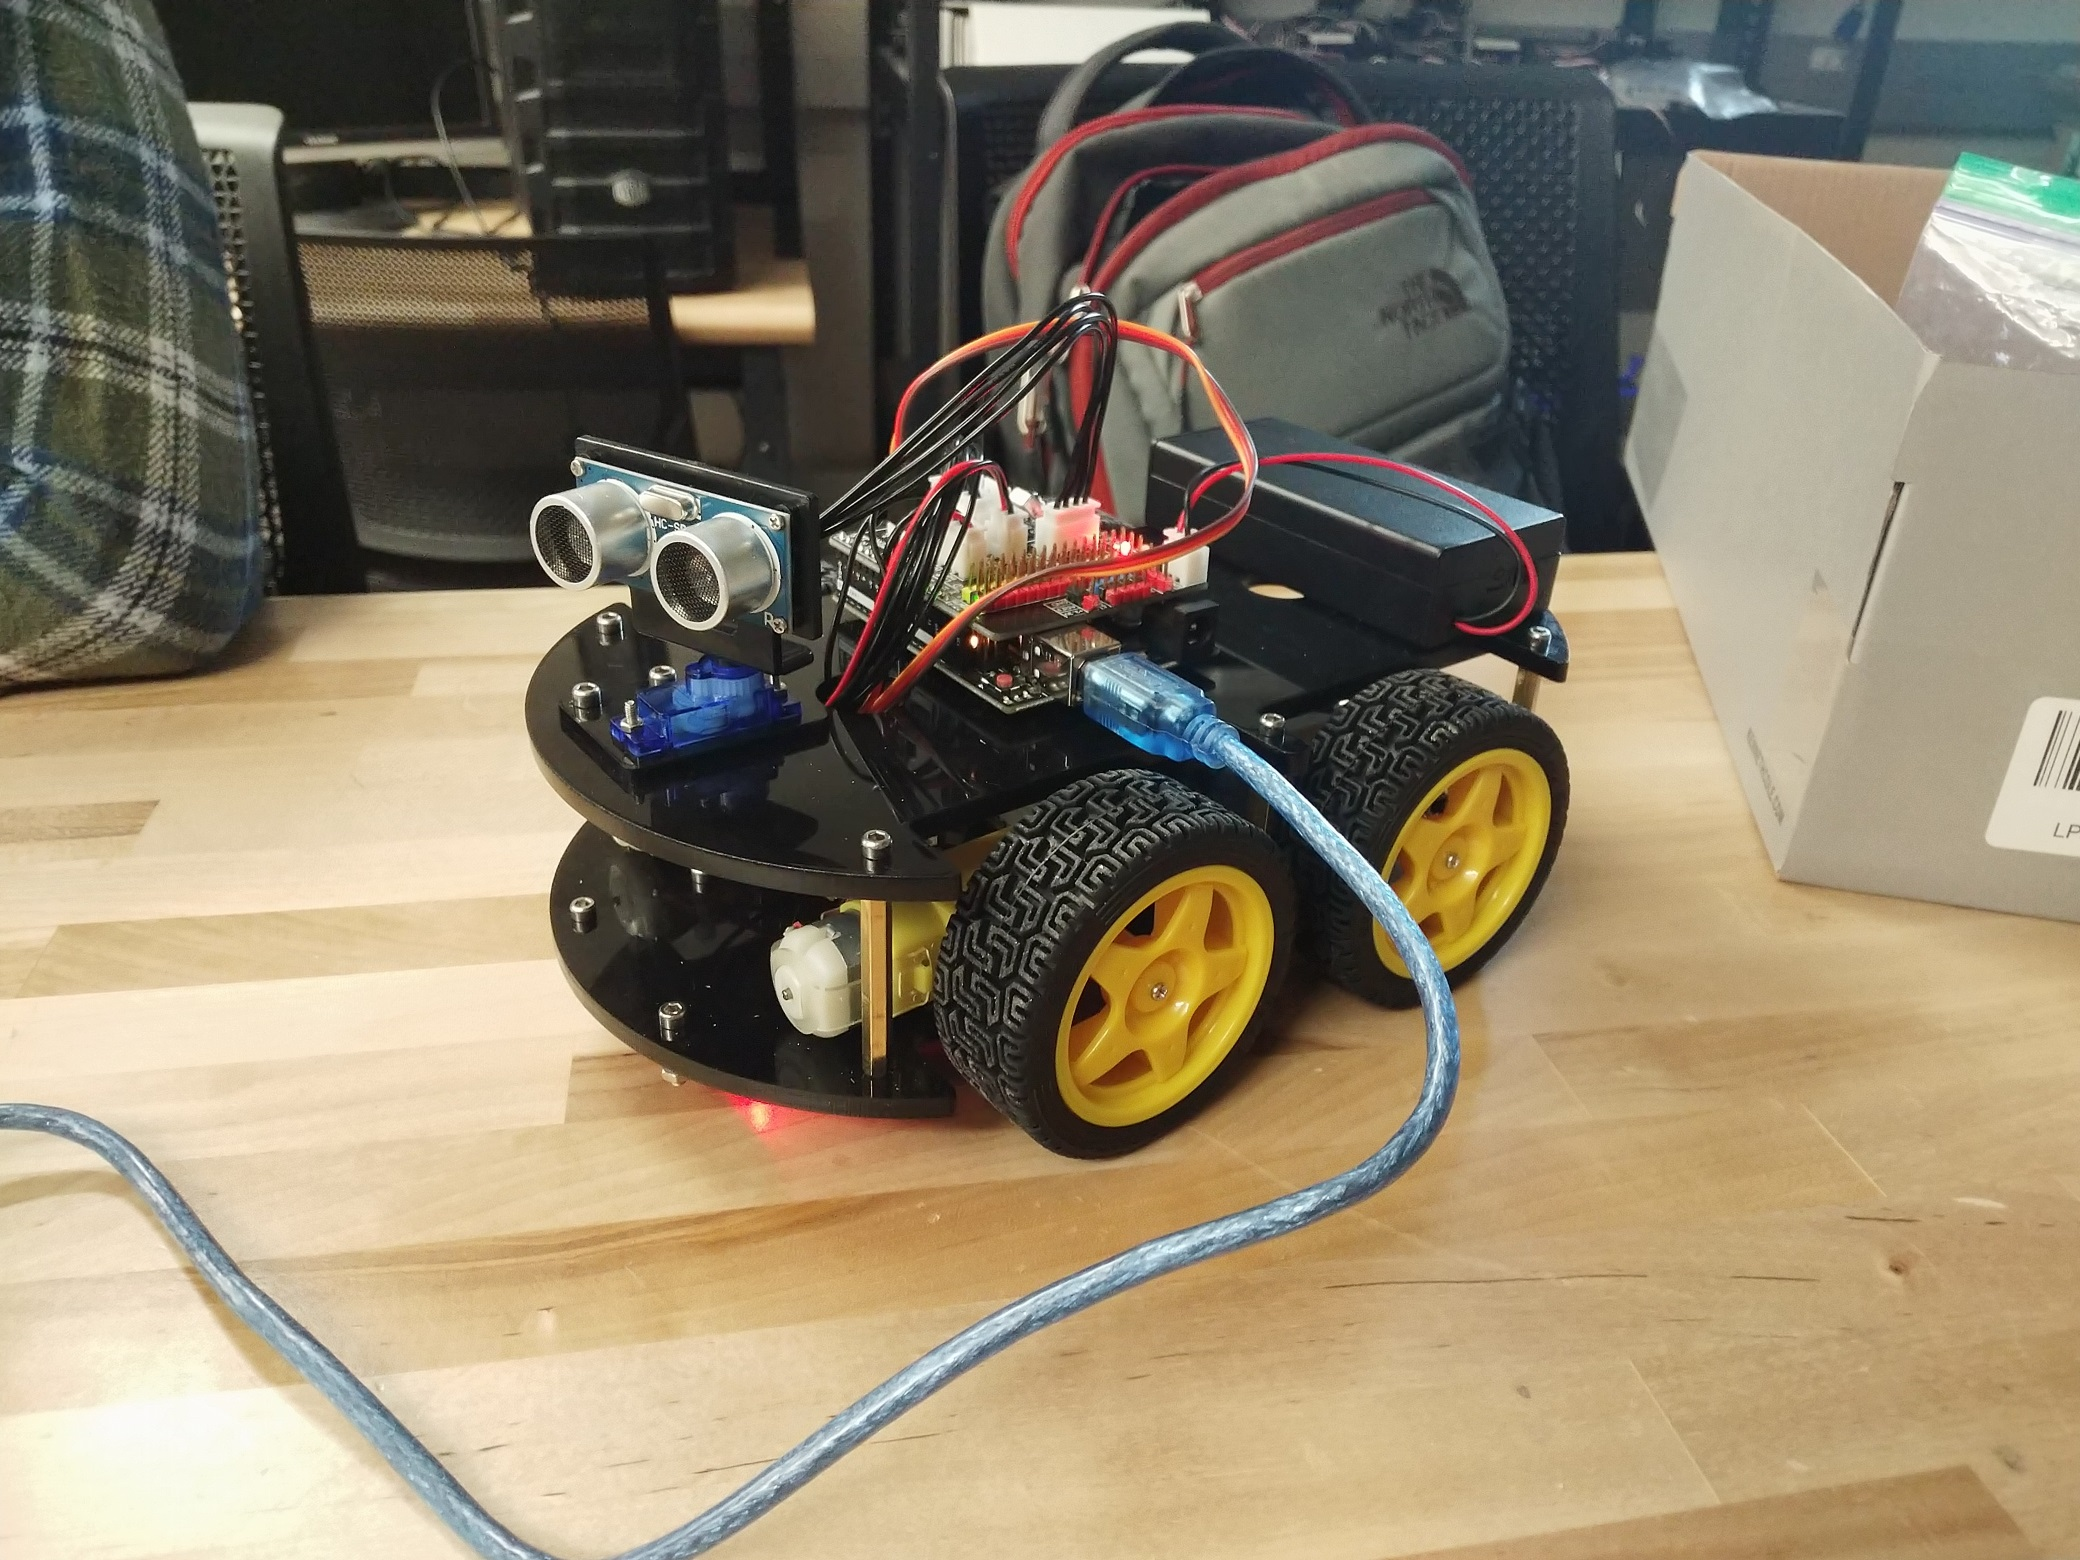
\includegraphics[width=\linewidth]{spare_me.jpg}
\end{center}
\caption{Fully assembled Elegoo robot car kit V3.0.}
\label{fig:f4}
\end{figure}

\section*{Implementation}
For this lab we are writing our own motor driver header and 
library which should allow us to use in the future. Because 
it also uses a pin map header file, we can also move the motor
headers around when needed.

\subsection*{initMotor}
All of our motor initializations with timer preperation and 
scaling, PWM modes and timer interrupt enable for turn functions.

\subsection*{setB}
Sets the OCR0B PWM pin and one side of our motor, specifically the 
left side motors on our robot. Set speed and direction with included 
enumeration inside of this motor driver file.

\subsection*{setA}
Sets the OCR0A PWM pin and one side of our motor, specifically the 
right side motors on our robot. Set speed and direction with included 
enumeration inside of this motor driver file.

\subsection*{turnLeft}
Simple abstraction function, activates the proper setB and setA functions 
with speed and length of time to be inside the function then stops.

\subsection*{turnRight}
Simple abstraction function, activates the proper setB and setA functions 
with speed and length of time to be inside the function then stops.

\subsection*{driveForward}
Simple abstraction function, drives the wheels forward for a set amount 
of time, then stops.

\subsection*{driveBackward}
Simple abstraction function, drives the whels backwards for a set amount
of time, then stops.

\subsection*{enum WHEEL\_DIRECTION}
Enumeration to allow ease of programming and simple calls for our motor driver
functions. Values are: 

\begin{itemize}
    \item forward
    \item back
\end{itemize}

\subsection*{delayUntilTargetCount}
% TODO

\subsection*{getNumInterruptsForDuration}
% TODO

\section*{Discussion}
Timers and motor drivers are finicky devices, especially on platforms with 
some degree of inaccuracy. By their inherent design DC motors are not entirely 
accurate but made to be fast and provide continuous drive. One of our first 
issues was in driving the motors and accounting for issues with the quality 
of the build, especially power distribution and toe, camber, and alignment of 
the wheels on their motors. Some degree of physical manipulation was performed 
but we ultimately took to software solutions to bias the wheels correctly by 
adjusting the PWM value written to the output compare registers.

Another issue was using the correct data type. On initial sketch we used integers, 
however, we later recalled that these are in fact 16 bit values being assigned to 
8 bit accurate registers. To prevent overflow, we changed these to 8 bit c-character 
variables immediately.

This lab is fairly straightfoward, using the OCR0X registers directly to write a 
relative speed between 0-255 in fast PWM mode on a 1024 prescale, we can more or 
less come to approximate to the easy mode Arduino IDE sketch of setting the digital 
pins PWM of 0-255. Then it's a matter of writing corresponding functions to 
make easier controlling the speed and direction to the motors.

\section*{Responses}
\begin{enumerate}
\item  PWM frequency for Timer 0 is controlled by the clock-select bits in TCCR0B. Test all five
PWM output frequencies while holding OCR0n static. What effects do you see on motor
speed/torque? Drawing on your knowledge from Circuits II, what is happening?

\item  Watchdog timers are a critical part of robust embedded systems. How do watchdog timers
function? Does the ATMega328P include a watchdog timer? If so, from where does it pull
its clock signal? To what value would one set WDTCSR if they wanted to reset the system
after one second of inactivity?

A watchdog timer is a timer that, when hitting a timeout, will attempt to reset the entire 
system. This is generally used to check for faults or large values of other timers and systems 
to prevent hanging of the entire system. It's generally good practice to reset or refresh the watchdog 
timer value at the end of certain processes to ensure it doesn't erroneously reset the entire system.

The ATMega328P does have a watchdog timer which pulls from it's own independent clock generator. One 
would set the last four bits of the WDTCSR register to 0110 for a one second watchdog timer.


\end{enumerate} 

\newpage
\section*{Appendices}
Table of contents:
\begin{itemize}
    \item main.c - entry, initialization and drive instructions
    \item bit\_macros.h - bit manipulations macros
    \item motor\_driver.h - header file for main motor driver
    \item motor\_driver.c - main c file for motor driver
    \item pin\_map.h - map of our motor pins
\end{itemize}
\newpage

\section*{Appendix A: main.c}
\begin{tiny}
\lstinputlisting{../main.c}
\end{tiny}
\newpage

\section*{Appendix B: bit\_macros.h}
\begin{tiny}
\lstinputlisting{../bit_macros.h}
\end{tiny}
\newpage

\section*{Appendix C: motor\_driver.h}
\begin{tiny}
\lstinputlisting{../motor_driver.h}
\end{tiny}
\newpage

\section*{Appendix D: motor\_driver.c}
\begin{tiny}
\lstinputlisting{../motor_driver.c}
\end{tiny}
\newpage

\section*{Appendix E: pin\_map.h}
\begin{tiny}
\lstinputlisting{../pin_map.h}
\end{tiny}
\newpage

\end{document}
\grid
